\newif\ifPAPER  
\PAPERtrue % select either slide or note
%\PAPERfalse  

\def\g4{{\sf Geant4}}

\newcommand{\codeAlgorithm}[1]{
\addcontentsline{toc}{section}{Résumé}
\begin{center}\fbox{\parbox{12cm}{\bf #1}}\end{center}}

\newcommand{\cppintro}[1]{
\lstset{language=C,
caption= #1 ,
label=listing:boundary}}

\def\cppstart{\begin{lstlisting}}
\def\cppend{\end{lstlisting}}

\newif\ifCITENOTE 
\CITENOTEtrue

\ifPAPER
\documentclass[twoside,floatfix,a4wide]{d}
\usepackage{multirow}
\usepackage{url}
\usepackage{listings}
\usepackage{graphicx}
\usepackage[utf8]{inputenc} % look here if scands are broken
\usepackage{wrapfig}
%\usepackage{makeidx}
\usepackage{subfig}
\usepackage{fancyhdr}
%\usepackage{asymptote}
\usepackage{amsmath}
\usepackage{verbatim} % for comment
\usepackage{eurosym} 
\usepackage{color} % for definecolor
\usepackage[colorlinks,bookmarks=true]{hyperref}

\numberwithin{equation}{section} % reguires amsmath-package
\pagestyle{fancy}
\fancyhead{} % clear all fields

\fancyhead[L]{\it {Helsinki, May 4, 2009}} % Left Odd, Right Even 
\fancyfoot[L]{G.Danielsen - Simulating carbon beam fragmentation on water phantom with the Geant4 INCL/ABLA models} 
\fancyhead[R]{\thepage}
\fancyfoot[C]{}
\newcommand{\urltilde}[1]{\texttt{#1}} % solves the tilde problem

\graphicspath{{images/}}
\DeclareGraphicsRule{.eps.gz}{eps}{.eps.bb}{`gunzip -c #1} % zipped images

\definecolor{light-gray}{gray}{0.95}
\definecolor{dark-gray}{gray}{0.30}
\definecolor{orange}{rgb}{1,0.5,0}
\definecolor{dark-blue}{cmyk}{1,0.5,0.5,0}
\hypersetup{
    bookmarks=true,         % show bookmarks bar?
    unicode=false,          % non-Latin characters in Acrobat’s bookmarks
    pdftoolbar=true,        % show Acrobat’s toolbar?
    pdfmenubar=true,        % show Acrobat’s menu?
    pdffitwindow=true,      % page fit to window when opened
    pdftitle={My title},    % title
    pdfauthor={Author},     % author
    pdfsubject={Subject},   % subject of the document
    pdfnewwindow=true,      % links in new window
    pdfkeywords={keywords}, % list of keywords
    colorlinks=true,        % false: boxed links; true: colored links
    linkcolor=dark-blue,          % color of internal links
    citecolor=dark-blue,        % color of links to bibliography
    filecolor=dark-blue,         % color of file links
    urlcolor=dark-blue            % color of external links
}
\begin{document}

\title{Simulating carbon beam fragmentation on water phantom with the Geant4 INCL/ABLA models}


\author{Gillis Danielsen$^1$ mentored by A.~Heikkinen$^2$} 
\affiliation{$^1$ Helsinki University of Technology}
\affiliation{$^2$ Helsinki Institute of Physics, P.O. Box 64, FIN-00014 University of Helsinki (Finland)}
\begin{titlepage}
\pagestyle{empty}
\begin{center}
rev. 001-2009\\
\vspace{7.5 cm}
\Huge
Simulating carbon beam fragmentation on water phantom with the Geant4 INCL/ABLA models\\

\vspace{5cm}

\Large
Gillis Danielsen, Bachelor's Thesis\\
Helsinki University of Technology\\

    \vspace{0,2cm}
  \end{center}

\end{titlepage}


\begin{abstract}
This work focuses on the simulation of carbon beams in a water phantom using GEANT4 code. Results will be compared to experimental data made available by the GSI Darmstadt/E.Haettner.

\footnote{Bachelor's thesis produced in the framework of the Finnish CERN Summer Training 2009.}
\end{abstract}
\maketitle
\thispagestyle{fancy}

\tableofcontents

\section{Introduction}

This paper focuses on the simulation of carbon beams in a water phantom using GEANT4 code as a medical application. GEANT4 is a multi-purpose physics simulation package developed at CERN, Switzerland. GEANT4 currently hosts multiple models suitable for the experiment, but this paper will focus on the INCL and ABLA models developed as a collaboration of scientists at CERN, GSI, HIP and CEA.

The history of radiation treatments dates back to the late 19th century when W.K. Roentgen discovered the X-rays. It was not long before these photon rays were being used to treat malign tissue. The first methods used were on today's standards very crude, and much work has gone into perfecting the treatments in order to minimize the effect of the rays on the surrounding healthy tissue and maximize the dose delivered to the malign tissue.

However, due to the statistical nature of the photon interactions, a beam of many photons is
exponentially attenuated yielding an exponential decrease of the dose with the depth. To
obtain a higher dose in the tumor than in the surrounding normal tissue, many irradiation
fields are used. The cost of this method is that a large volume of the normal tissue
will suffer from a high dose. By replacing the x-rays with high energy photons, the dose
maximum is shifted a few centimeters deeper and the exponential decrease is more shallow,
which improves the ratio between dose in the tumors and in the normal tissue.

Although very sophisticated variations of the photon treatments have been perfected over time, photon therapies still produce considerable harm to the surrounding tissue. A much younger and less widely used technology are those of hadron- or heavy-ion based radiotherapies. Hadrons and heavyer-ions are charged particles and therefore react to tissue in a much different way to photons. The dose-profile contains a much sharper peak due to the primary halting force being electromagnetic interaction. This peak is called the bragg-peak, and was first discovered by William Henry Bragg in 1903.

The field of hadron treatments were pioneered by Berkeley. Based on research done at the Berkeley cyclotron J.Wilson first recomended the use of protons as a treatment method in a 1946 paper ~\cite{RW46}. Furthermore, the first de facto treatment was administered at Berkeley in 1953. Today there are is a number of proton-based therapies in clinical use around the world.

Heavy-ion therapies have remained considerably less common and have remained on a more experimental level. Clinical trials were conducted at Lawrence Berkeley Laboratory (LBL) inbetween 1977 and 1993 with $Ne_20$. At the end of 2008 PTCOG estimated that more than 7000 heavy-ion treatments had been conducted at treatment facilities it monitors worldwide . Treatments based on $^{12}$C beams have been offered at NISR in Japan and in Germany at GSI.~\cite{PTCOGstat}

The motivations for heavy-ion treatments as an alternative or complement to hadron treatments are considerable. Firstly carbon ions have the added advantage of higher ionisation-density at the end of their range, causing greater correlated damage to the DNA-structure of a single cancerous cell and therefore induces damage in a way that makes it less likely the cell is able to repair itself. In a 2008 article O.Jäkel ~\cite{ojakel} approximates the beam's increase in biological efficiency by a factor between 1.5 and 3 depending on the application in comparison to proton treatment. Secondly, Heavy-ions ions are less scattered in lateral directions which yields better dosage control in many applications. However, the tradeoff is that carbon-ions will fragment into smaller particles, yielding an unwanted ``tail`` to the energy-loss profile. One of the main motivations of the work is to study this ''tail'' for the ``worst case scenario'' of 400 MeV - an upper limit seldom crossed in medical applications.

A number of data-sets are available for carbon beams. This paper will be compare data to beam-measurments by E. Haettner ~\cite{ehaettner}  at the GSI facility in Darmstadt, Germany. This paper intends therefore to mimic the experimental setup used by E.Haettner. The aim of this paper is  to provide good reference data for the standardization work involved in hadron treatments and to evaluate the feasibility of the GEANT4 models for such simulations by comparison to experimental data.

\section{Theory}

\subsection{Electromagnetic physics of Bragg-curve}
As charged particles cross tissue they interact with the particles in the tissue through elastic and inellastic collisions with the electrons and nuclei, eventually loosing all of its energy. The largest contribution comes from inellastic collisions with electrons, contributing as much as 99 percent of the total energy loss.

The beam's energy loss as a function of depth is called the Bragg Curve. Theoretical estimates for this relation have existed since the first classical treatment by Bohr in 1913~\cite{bohr13}. The currently used quantum model was derived by Bethe and Bloch in 1953~\cite{bethebloch53}  and is commonly known as "Bethe's stopping power formula". The Bethe stopping power formula is generally considered a good model for most swift charged particles, with the exception of electrons.

\begin{equation}
 \frac{dE}{dx} = \frac{4 \pi}{m_e c^2} \cdot \frac{nz^2}{\beta^2} \cdot \left(\frac{e^2}{4\pi\varepsilon_0}\right)^2 \cdot \left[\ln \left(\frac{2m_e c^2 \beta^2}{I \cdot (1-\beta^2)}\right) - \beta^2\right],
\label{bethebloch}
\end{equation}
where $\beta = v/c $, 
$v$ is the velocity of the particle ,
$E$ is the 
energy of the particle,
$x$ is the 
distance travelled by the particle,
$c$ is the 
speed of light,
$z\,e$ is the 
particle charge,
$e$ is the 
charge of the [[electron]],
$m_e$  is the 
rest mass of the electron,
$n$ is the 
electron density of the target and 
$I$  is the 
mean excitation potential of the target.


However, as the speed of the particle has decresed to the order of magnitude of the Bohr velocity the nuclear charge $Z_P$ will no longer remain constant and has to be aproximated by the effective charge, given by the Barkas formula $Z_{P_eff} = Z_{P}(1-exp(-125\beta_{P}Z_{P}))$.

In this theoretical model the Bragg-peak can be understood as the $1/v_{p}^2$ relation increases the energy-loss as the speed decreases. However, the effective charge will decrease at an exponential rate and thus converge the Bragg-curve.

Particles crossing matter do not just deposit energy through inelastic electron collisions, they might as well be involved in nuclear reactions and fragmented. A common textbook physical model for explaining this is called the abrasion-ablation model. In this model high
energy projectiles can be described as particles that move on straight lines through the
target and from time to time a target nucleus lies on this line and causes a collision. Bullet
and target nucleons which overlay eachother in the collision are called participants,
while the remaining parts of the projectile and target nucleus are called spectators. Spectators in the projectile are only slightly affected by the collision, while spectators in the target stay at rest. The participant nucleons form an excited entity, or ``the fireball'' which fragments into light ions or single nucleons. This kind of a model is however not directly comparable to the model used in this paper through INCL and ABLA. The Wilson-model that also is bundled with Geant4 features a physics model more reminiscient to this approach.
\begin{figure}
\begin{center}
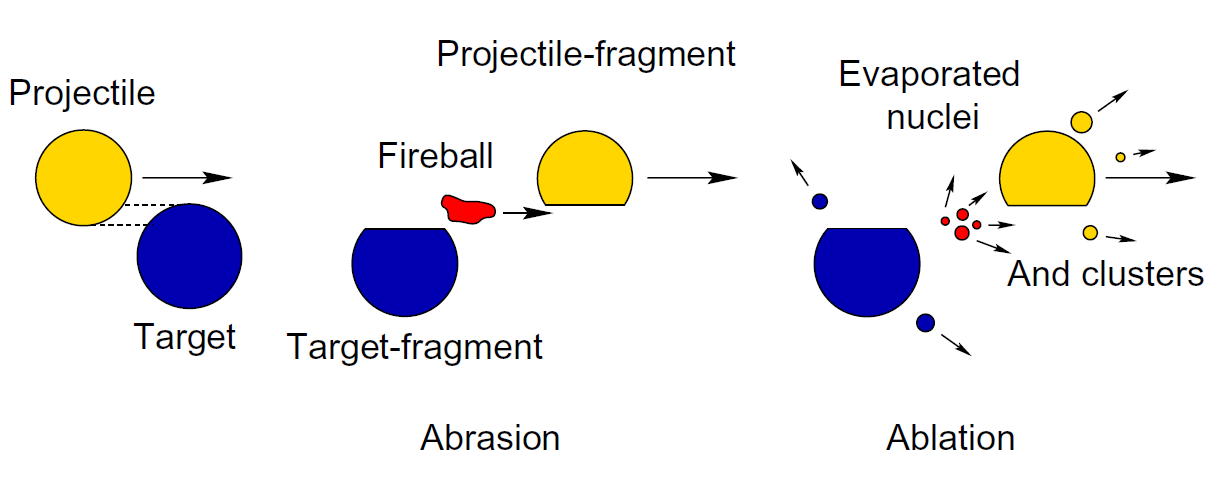
\includegraphics[width=0.8\textwidth]{images/ablationabration.png}  
\caption{Schematic description of abration-ablation model. (Wilson model in Geant4)}
 \label{fig:ablationabration}
 \end{center}
 \end{figure}



\subsection{INCL and ABLA models} %theory, no practical aspects



INCL is a Monte-Carlo type Intranuclear Cascade Model, whereas ABLA is the the complementing Monte-Carlo evaporation/fission model. In practice this means INCL is used to determine what happends just after the the ``bullet'' particle hits the nucleus, while ABLA is used to determine what nuclear process is caused through the following excitation of the target due to the collision event. It is notable that the time-frame for evaporation and fission events are orders of magnitude greater compared to the events processed by INCL.


\begin{figure} 
\begin{center}
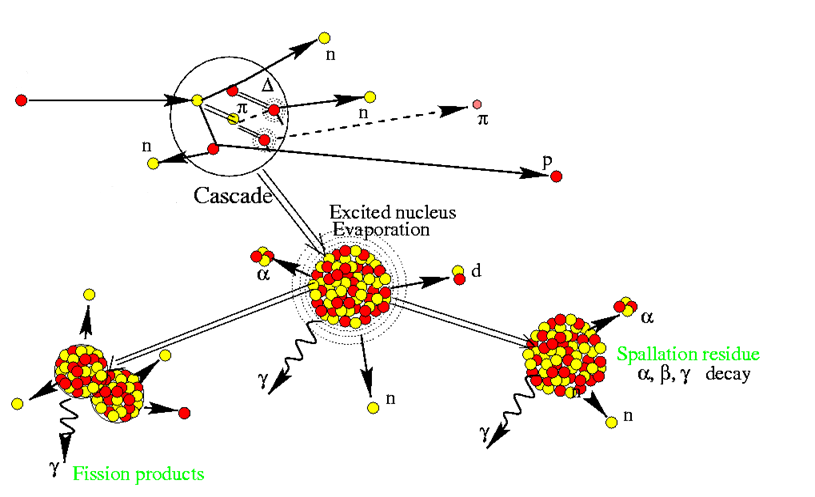
\includegraphics[width=0.8\textwidth]{images/inclScematic.png}  
\caption{\label{fig:inclschematic} Schematic diagram of INCL and ABLA models.}
 
 \end{center}
 \end{figure}


\subsubsection{INCL}

INCL is developed from the on Liege cascade, but contains less free parameters in order to improve certain discrepancies in the Liege code. INCL is designed for use in the 200MeV-2GeV where standard cross-section libraries no longer are sufficient.

INCL is called into action when Geant4 stochastically determines an inellastic collision will take place. INCL then takes as parameters the beam-particle and the target nucleus given to it by Geant4. It then proceeds to stochastically determine what type of collision will happen by randomly picking the impact parameter between zero and the the target nucleus radius. The impact parameter is defined as the perpendicular distance between the velocity of the projectile and the center of the nucleus it is approaching.

INCL is a model where particles move in straight deterministic trajectories, which makes operation fast as the upcomming collisions are easy to predict. The nucleus in INCL is modelled as fermi-gas in a Woods-Saxon potential. The Woods-Saxon potential barrier gives a potential barrier that is smooth, and also means the nucleons are randomly picked from the Woods-Saxon type probability density-distribution.

\begin{equation}
\rho(r) = \begin{cases}
\frac{\rho_{0}}{1+\exp({\frac{r-R_{0}}{a}})} & 0 < r < R_{max} \\
0 & \text{otherwise}
\end{cases}
\label{WoodsSaxon}
\end{equation}

If the energy of the bullet particle breaks the nucleus potential barrier and enters the nucleus several binary collissions between participator nucleons will take place, and smaller particles may be errupted. Spectator particles may move around the nucleus and bounce off it's edges, but they will not leave the nucleus.

The kinetics of the model are bound by the physical laws of conservation of baryon number, charge, energy, momentum and angular momentum and respect for the Pauli blocking principle. Furthermore pion-production is governed through the relation of $NN \rightleftharpoons N\Delta, \Delta \rightleftharpoons N\pi$ (with a stochastically determined mass for $\Delta$).

The major free parameter of the INCL model is the stopping-time, that is, how long the model be used before thermal equilibrium can be assumed and thus the process handed over to the evaporation and fission model. The INCL code has chosen the stopping time as a suitable function of the target nucleus size so that $t_{stop} = f_{stop}t_0(\frac{A_T}{208})^.16$, where $f_{stop}$ will be left at the default of 1.0 in this work. The stopping-time of INCL is considerably longer than for many models where discrete potential barriers are defined for the nucleus.

For the scope of this paper a further discussion of the theoretical basis of INCL is deemed unneccessary but the interested reader may find the following sources valuable. ~\cite{PhysRevC.66.044615} ~\cite{iia}

\subsubsection{ABLA}

The ABLA code was developed over many years at the GSI facility in Darmstadt, Germany principally by Karl-Heinz Schmidt and Aleksandra Kelic. It is a Monte-Carlo code based on a large data-set distributed that is distributed alongside the code. ABLA takes as input nucleus parameters, excitation energy, mass number, charge number and nucleus spin. It then calculates on the basis of this data the probabilities for different fission or fragmentation events to take place according to the stored static statistical distributions obtained from experiments or phenomenology.

ABLA comes with two different fission models SimFis3 and SimFis18. These models are based on the proven PROFI-model also developed at GSI darmstadt.

SimFis3 features


\section{Simulation setup} %practical aspects of simulation
The simulation is to be performed with the latest versions of the INCL and ABLA code that is a part of the GEANT4 suite.

\begin{itemize}
\item Experiment data from GSI
\item target description
\item Characterization of the beam
\item Simulation of detectors
\item Implementation details
\end{itemize}

\subsection{Improving usability through messenger macro commands}
The first action task taken in this work was to implement means of saving analysis files with a user-defined name.

So as aen example the user can give a command according to the following syntax.
\scriptsize
\begin{verbatim}
/analysis/setFileName <user-defined name>.root
\end{verbatim}
\normalsize

The implementation was done by creating an analysismessenger inheriting functionality from \textit{G4UImessenger}. An object of the type \textit{HadrontehrapyAnalysisMessenger} was created in the \textit{AnalysisManager}.


\scriptsize
\begin{verbatim}
class HadrontherapyAnalysisFileMessenger: public G4UImessenger
{
  public:
    HadrontherapyAnalysisFileMessenger(HadrontherapyAnalysisManager*);
   ~HadrontherapyAnalysisFileMessenger();
    
    void SetNewValue(G4UIcommand*, G4String);
    
  private:
    HadrontherapyAnalysisManager* AnalysisManager;
\end{verbatim}
\normalsize
\begin{figure} 
\begin{center}
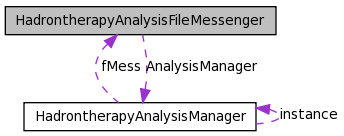
\includegraphics[width=0.3\textwidth]{images/setFileNameMessenger_1.png}  
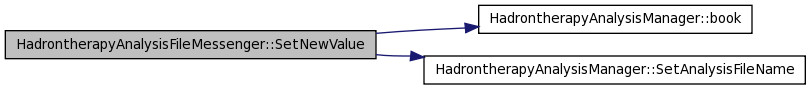
\includegraphics[width=0.7\textwidth]{images/setFileNameMessenger_2.png}  
\caption{\label{fig:messengerUML} UML diagrams for messen ger class}
 
 \end{center}
 \end{figure}

\section{Results and comparison to GSI data}
\begin{itemize}
\item comparison (Haettner 5.4.1)
\item energy distribution of fragments
\end{itemize}

\section{Conclusion}
\begin{itemize}
\item Raflaava yhteenveto
\end{itemize}

\section{Appendices}
\begin{itemize}
\item code examples
\item runtime log
\end{itemize}





\bibliographystyle{plain} \bibliography{refs.bib} 
\end{document}

\else

\fi